\documentclass[10pt]{iopart}

\usepackage{graphicx}
\graphicspath{{./figures/}}
%\usepackage[acronym]{glossaries}
\usepackage{acro}

\DeclareAcronym{cejst}{short=CEJST,
                       long=Climate and Energy Justice Screening Tool
}

\DeclareAcronym{ipcc}{short=IPCC,
                      long=International Panel on Climate Change
}

\DeclareAcronym{nsrdb}{short=NSRDB,
                       long=National Solar Radiation Database
}

\DeclareAcronym{nrel}{short=NREL,
                       long=National Renewable Energy Laboratory
}

\DeclareAcronym{lmi}{short=LMI,
                     long=low and moderate income
}

\DeclareAcronym{uhi}{short=UHI,
                     long=Urban Heat Island
}

\DeclareAcronym{ceja}{short=CEJA,
                      long=Climate and Equitable Jobs Act
}

% \usepackage[numbers]{natbib}
\usepackage{cite}
\usepackage{tabularx}
\usepackage{float}


\begin{document}

\title[Minimizing heatwave risk through an equitable distribution of solar panels]{Minimizing
heatwave risk through an equitable distribution of solar panels}

 \author{
 Samuel G. Dotson$^1$$^*$,
 Shannon R. Anderson$^2$,
 Alankrita Sahay$^3$,
 Pranjali Borse$^3$,
 Charumeghana Samantula$^3$
 }

 \address{ $^1$ Department of Nuclear, Plasma, and Radiological Engineering,
 University of Illinois Urbana-Champaign, Urbana IL, United States}
  \address{ $^2$ Department of  Natural Resources and Environmental Sciences,
 University of Illinois Urbana-Champaign, Urbana IL, United States}
  \address{ $^3$ Department of Civil and Environmental Engineering,
 University of Illinois Urbana-Champaign, Urbana IL, United States}
 \address{$^*$ Author to whom correspondence should be addressed}

 \ead{sgd2@illinois.edu}

 \begin{indented}
 \vspace{10pt}
 \item[]May 2022
 \end{indented}

 \begin{abstract}
 Testing abstract. \ac{cejst}. \ac{cejst}
 \end{abstract}

 \vspace{2pc}
\noindent{\it Keywords}: solar, heatwave, equity, energy justice, policy

\ioptwocol
\acresetall

\section{Introduction}
Climate change will increase the frequency and severity of extreme heat events and,
due to the \ac{uhi} effect, urban centers are more susceptible to heat waves and
heat stress \cite{zhao_strong_2014,dahl_killer_2019}. The Union of Concerned
Scientists estimates that the number of days above 32 $^\circ$C in the Midwest
will increase five-fold by midcentury unless action is taken to reduce carbon
emissions and slow climate change  \cite{dahl_killer_2019}. The lack of strong
federal climate policies leaves individual states and institutions responsible
for acting on climate change. Illinois passed the \ac{ceja} in 2021 which established
strong climate goals and programs for the state, including subsidies for rooftop
solar panels \cite{harmon_climate_2021}. This case study investigates the optimal
distribution of rooftop solar panels that minimizes heat wave risk for the City of
Chicago.

We chose Chicago as the focus of this work for two reasons. First, Chicago was the
epicenter of a deadly heat wave in 1995; one of the deadliest heat waves in United
States history. Over 700 people died in this heat wave\cite{klinenberg_heat_2003}.
Further, the death toll from this heat wave was exacerbated by a combination of
social factors including income, isolation, and crime rates \cite{klinenberg_heat_2003}.
As a result of this heat wave, Chicago officials recognized the need to prepare
for future heat waves. This
work proposes rooftop solar panels as a possible mitigation strategy.
Second, the State of Illinois has programs such as Solar for All and Illinois
Shines that aim to provide greater access to clean energy for low-income populations
\cite{illinois_solar_for_all_environmental_2022}. Thus, the resources to increase
rooftop solar penetration already exist but lack guidance based on heat wave risk.

Illinois Solar for All and Illinois Shines are two programs strengthened by the
2021 \ac{ceja} bill \cite{harmon_climate_2021,illinois_solar_for_all_environmental_2022}.
These policies intend to expand the rooftop solar capacity in Illinois by providing
incentives or subsidies for solar installation, with specific allocations for
low-income communities. Rooftop solar
panels help reduce the percentage of household income spent on energy costs,
known as the energy burden, through net-metering policies that pay consumers for
excess energy generation \cite{brown_high_2020}. This reduction of energy burden
improves resilience to heat waves by increasing access to air-conditioning for
low-income households during high-demand times when electricity is most expensive.
However, a high penetration of intermittent renewables, such as solar panels,
increases price volatility and the energy burden for consumers without solar
installations \cite{rai_impact_2020,johnathon_analyzing_2021}. This is called the
``paradox of renewable energy policy'' and highlights the need for efficient
prioritization of at-risk areas \cite{blazquez_renewable_2018}.
Therefore, the purpose of this study is to identify areas with the highest heat
wave risk so they may be prioritized by programs like Solar for All and Illinois
Shines.

In order to identify high-priority areas, we curated economic and demographic
data for Chicago, along with satellite data from the \ac{nsrdb} published by the
\ac{nrel}. We identified regions of similar risk and suitability for solar panels
with a hierarchical clustering algorithm. Section \ref{section:methods_data}
discusses details of the data selection and processing, section \ref{section:results}
presents the results of the clustering algorithm, and section \ref{section:discussion}
develops a descriptive typology based on the clustered areas.


\section{Literature Review}
The \ac{uhi} effect, where urban areas tend to be warmer than their surroundings,
is among the most well studied phenomena, often using remote sensing technology and land
surface temperature data \cite{almeida_study_2021, cotlier_extreme_2022}.
Some studies evaluated \ac{uhi} intensity for particular cities by incorporating
data about urban features such as albedo, building height, and vegetation
\cite{sangiorgio_development_2020,abulibdeh_analysis_2021} along with urbanization
trends \cite{li_how_2021}. Other work in the literature examined \ac{uhi} along
a socio-economic axis. Chakraborty et al. \cite{chakraborty_disproportionately_2019}
used satellite and census data for multiple cities and found that \ac{uhi}
disproportionately affects low-income residents in most places, including Chicago,
and suggest that \ac{uhi} mitigation should benefit demographic groups that experience
greater \ac{uhi} intensity. Hsu et al. \cite{hsu_disproportionate_2021} also
found that race and income level were correlated with greater \ac{uhi} intensity.

Strategies to mitigate \ac{uhi} typically interrupt the heat storage process that
drives \ac{uhi}, where
low albedo surfaces such as pavement and rooftops absorb and trap heat. Green roofs
are a popular method to reduce \ac{uhi} by reducing heat storage and increasing
the energy from latent heat rather than sensible heat \cite{zhang_effectiveness_2017}.
Similar to green roofs, several studies determined that increasing the urban
tree canopy is an effective way to reduce \ac{uhi} by reducing heat storage in
surfaces, but also by providing shade \cite{middel_urban_2015,
loughner_roles_2012, mcdonald_tree_2021, marando_urban_2022, schwaab_role_2021}.
``Cool'' roofs reduce \ac{uhi} by increasing the albedo of rooftop surfaces and
decreasing the amount of radiation that gets absorbed \cite{zhang_effectiveness_2017,
salamanca_citywide_2016, middel_urban_2015}. Lastly, rooftop solar panels are also
found to, counter-intuitively, mitigate \ac{uhi} effects at night due to boundary
layer structure and by reducing energy requirements for cooling \cite{masson_solar_2014,
sailor_photovoltaics_2021, salamanca_citywide_2016}. However, the primary
function of solar panels is to improve adaptive capacity by generating energy
for cooling \cite{masson_solar_2014}.

As with \ac{uhi} intensity, the literature also indicates that \ac{uhi} mitigation
efforts disproportionately benefit wealthier residents. McDonald et al. reported
that high-income areas had nearly twice the tree canopy of neighboring low-income
regions \cite{mcdonald_tree_2021}. Further, efforts to mitigate \ac{uhi} with
vegetation may lead to gentrification, thereby excluding the intended beneficiaries
\cite{chakraborty_disproportionately_2019}. Solar panel adoption has also developed
along socio-economic lines. Vaishnav et al. \cite{vaishnav_was_2017} showed that
subsidies for rooftop solar panels favored the affluent. Reames et al.
\cite{reames_distributional_2020} identified that the greatest solar panel
penetration was found in areas with the greatest income, although it remained
quite low compared with other cities. The researchers also indicate that lack
of information contributes to these disparities \cite{vaishnav_was_2017,reames_distributional_2020}.
Illinois' Solar for All campaign sought to prioritize low-income areas using a
tool called the \ac{ejscreen} from the \ac{epa} \cite{us_epa_ejscreen_2014}. Another
tool that identifies climate justice areas is the \ac{cejst}
\cite{council_on_environmental_quality_climate_nodate}. However, neither of these
tools incorporate temperature data nor \ac{uhi} effects, thereby limiting their
effectiveness at targeting areas facing heat wave risk.

In the present work, we use the hazard-exposure-vulnerability framework for
risk established by \ac{ipcc} in 2018 \cite{viner_understanding_2020}. This
framework is useful for understanding the different factors that contribute to
risk. Hazards are the climate events that can produce adverse outcomes. Examples
include flooding, hurricanes, and heat waves. Our work focuses on the latter.
Exposure implies the presence of people. People are not at risk from a hazard if
they are not present. Regions with different population densities have different
levels of exposure. Further, cities have a higher exposure to heat waves due to
\ac{uhi}. Lastly, vulnerability describes susceptibility and adaptive capacity to
particular hazards. This includes socio-economic factors such as race, income,
and age. Adaptive capacity reduces exposure or vulnerabilities while mitigation
efforts minimize the hazard itself.

As identified earlier, lower income is associated with greater \ac{uhi} and therefore
both a greater exposure to heat waves with less adaptive capacity. However, income
is one of many factors that contribute to heat wave risk. Maragno et al.
\cite{maragno_mapping_2020} mapped heat stress risk by adapting the
hazard-exposure-vulnerability framework and included age as a demographic vulnerability
along with landuse for different types of buildings. There are other
socioeconomic factors that contribute to heat wave risk, such as crime rate,
educational attainment, access to cooling centers, and housing characteristics
\cite{klinenberg_heat_2003,gronlund_racial_2014} that Maragno et al. do not include.

Several works mapped regions with the highest \ac{uhi} \cite{almeida_study_2021},
identified disparities in \ac{uhi} \cite{chakraborty_disproportionately_2019} and
its mitigation \cite{reames_distributional_2020, mcdonald_tree_2021}. At least one
study applied the hazard-exposure-vulnerability framework in a heat wave risk
assessment \cite{maragno_mapping_2020}. However, there is no existing literature
that prescribes a methodology for efficient allocation of rooftop solar panels.
The present work fills that gap by collecting satellite and socio-economic data
to identify areas of high heat wave risk that accounts for disparities in
exposure and adaptive capacity.


% \begin{itemize}
%   \item What studies have mapped uhi?
%   \item What papers have looked at uhi and class?
%   \item What papers have looked at uhi mitigation strategies?
%   \item What are the most frequent mitigation strategies (green+white roofs)
%   \item What papers have looked at the solar panel distribution?
%   \item What are the social aspects of solar panel distribution?
%   \item How have solar panels been distributed previously? (Introduce CEJST \& EJSCREEN)
%   \item What gap in the literature is this work specifically filling?
%   \item How are we defining risk? solar panels may worsen the hazard since they have a low albedo.
% \end{itemize}
%
%
%
%
% Various studies have addressed heat wave problem and distribution of solar panels separately till now. An assessment by means of Land Surface Temperature using remote sensing technology \cite{cotlier_extreme_2022}, the mapping of heat stress by crowdsourcing geospatial data and high spatial resolution data and evaluation of socioeconomic characteristics \cite{maragno_mapping_2020}, quantifying synergies between Urban Heat Island effect and heatwaves in urban areas \cite{founda_synergies_2017}  are some of the studies addressing heatwave problem. While these studies mainly discuss about the spatial distribution of heat stress, others have also addressed its implications to the society by assessing socio-economic vulnerability and risk. One of the study\cite{maragno_mapping_2020} has developed sensitivity, adaptive capacity, vulnerability, exposure, and risk indicators and tested the framework on urban area concluding that vulnerability and risk levels differ with changing locational characteristics within the same urban area and hence the high resolution spatial dataset serves a great importance to plan necessary adaptation strategies. This study served as a foreground to choose the high resolution datasets in our study. Our study area is Chicago city which is an highly urbanized area with varying locational characteristics. We reviewed few studies related to Chicago heatwaves. The study by Bernice Ackerman  has addressed the effect of Lake Michigan on temperature of its surrounding area and the effect of green cover. It was helpful in identifying the crucial indicators like green cover and presence of water bodies which help surrounding areas to stay relatively cooler and hence could serve as good adaptive capacity indicators.
%
% Prior research has shown works that study the distributional disparities in residential rooftop solar potential in four major cities in Chicago and a few other cities \cite{reames_distributional_2020}. The study found that the highest rooftop potential in Chicago was in census tracts with higher percentages of \ac{lmi} households. The \ac{lmi} households represented 51\% of solar suitable households in Chicago. However, the lower penetration of solar \ac{lmi} communities substantially decreases the overall attainment of renewable energy and energy equity goals in Chicago.  DeepSolar, a machine learning framework that efficiently constructs a solar deployment dataset for the United States has found that the solar deployment density is strongly correlated and decreases with the Gini index, a measure of income inequality \cite{yu_deepsolar_2018}. This points out how socio-economic inequality causes disparities in solar distribution. Most states across the United States have developed one or more policies to incentivize distributed solar PV investments. Many states have adopted various additional financial incentives to encourage and support the deployment of customer-owned distributed solar energy systems \cite{pitt_assessing_2015}. These policies and incentives are similar to Illinois Shine and Solar for All programs in Illinois which the current study focuses on.
% However, it has also been shown that the distribution of low-carbon technology subsidies and their associated benefits can be highly uneven across socioeconomic groups, revealing a persistent inequality issue. The high income community usually have the resources and knowledge required to avail the benefits of such subsidies and hence tend to be more benefited than their low income counterparts \cite{stewart_all_2021}. This escalates the need for equitable distribution of the solar incentives across different socioeconomic communities. Hence, this study aims to find the ‘high risk’ areas in Chicago and help facilitate equitable distribution of solar panels through the Illinois Shine and Solar for all programs.


\section{Methods and Data}
\label{section:methods_data}
In this section we review the data we collected for the City of Chicago and the
methods we used to cluster Chicago's census tracts into priority areas for solar
panel distribution. We used the hazard-exposure-vulnerability framework asserted
by the \ac{ipcc} to categorize the datasets used in this work
\cite{viner_understanding_2020,field_determinants_2012}.


\begin{table}[H]
  \centering
  \caption{Summary of curated data for the city of Chicago}
  % \begin{indented}
  \begin{tabular}{lllll}
    \br
    Dataset & Risk Aspect & Spatial & Factor & Source \\
     & Aspect & Resolution && \\
     \mr
     Temperature & Hazard & Community Area & Aggravating & \cite{sengupta_national_2018}\\
     Population density & Exposure & Census tract & Aggravating & \cite{city_of_chicago_boundaries_nodate}\\
     Percent tree canopy & Vulnerability & Community area & Mitigating & \cite{kua_chicago_2020}\\
     Energy burden & Vulnerability & Census tract & Aggravating & \cite{council_on_environmental_quality_climate_nodate}\\
     Age & Vulnerability & Census Tract & Aggravating & \cite{city_of_chicago_boundaries_nodate}\\
     Cooling centers & Vulnerability & Community Area & Mitigating & \cite{city_of_chicago_boundaries_nodate}\\
     Social network & Vulnerability & Community Area & Mitigating & \cite{city_of_chicago_boundaries_nodate}\\
     Crime rate & Vulnerability & Community Area & Aggravating & \cite{city_of_chicago_boundaries_nodate}\\
     Percent qualified roof area & Vulnerability & Census Tract & Mitigating& \cite{google_project_2022}\\
     \br
  \end{tabular}
  % \end{indented}
\end{table}

\subsection{Hazard}

Hazards are the climate-related events the may lead to adverse outcomes for people,
such as losses of life, function, property, infrastructure, and resources
\cite{viner_understanding_2020}. In this work, we focus on the risk of heat stress
and the potential for heat-related deaths, for which temperature is the primary
hazard. We gathered hourly temperature data for each community area in Chicago for the
years 2000 to 2020 using the \ac{nsrdb} \cite{sengupta_national_2018}. In order
to capture the temperature difference among Chicago's community areas during heatwaves,
we set a temperature threshold of 32$^\circ$C and filtered out the data below this
threshold. We defined a heatwave temperature anomaly,
\begin{eqnarray}
  H_a = T_{ca} - T_{city},
\end{eqnarray}
where $T_{ca}$ is the temperature of the community area and $T_{city}$ is the
mean temperature of the city (i.e. the mean of all community areas), in celsius.
We then took the mean of the hourly $H_a$ to use in our clustering algorithm.
Figure \ref{fig:ha_map} shows the variations in temperature during heatwaves in
Chicago.

\begin{figure}[H]
  \label{fig:ha_map}
    \begin{center}
      \includegraphics[width=\columnwidth]{temperature_anomaly_map}
      \vspace*{-2cm}
      \caption{The temperature variations among community areas in Chicago during
      heatwaves. Higher values indicate warmer temperatures than the city mean
      temperature and lower values indicate cooler temperatures.}
    \end{center}
\end{figure}

A greater $H_a$ indicates regions that experience higher temperatures during
heatwaves and lower a $H_a$ indicates regions with lower heatwave temperatures.
The region near O'Hare International Airport experiences the highest temperatures,
nearly 2$^\circ$C above the citywide average. The temperature anomalies are further
adjusted by subtracting the minimum temperature difference such that the
coolest area of the city has an $\bar{H_a}$ value of zero and other values indicate
the temperature above this minimum value. This is done to ensure good behavior
from the clustering process.

\subsection{Exposure}

Exposure is the presence of people or important assets in places that could be
adversely affected by climate hazards \cite{viner_understanding_2020}.

\subsection{Vulnerability}

Vulnerabilities are the factors that predispose certain groups or areas to adverse
outcomes. We consider several physical and social vulnerabilities. There are several
works that map the potential for heat stress, 

\subsubsection{Energy Burden}

Energy burden is the ratio of household energy costs to household income. We
used data from \ac{cejst} to create a map of energy burden in Chicago
\cite{council_on_environmental_quality_climate_nodate}. Energy
burden affects access to electricity, especially during heatwaves when demand
and cost of electricity are highest. Rooftop solar panels can reduce energy costs
and therefore improve access to cooling during heatwaves. Figure \ref{fig:eb} shows
the distribution of energy burden throughout Chicago.

\begin{figure}[H]
  \label{fig:eb}
    \begin{center}
      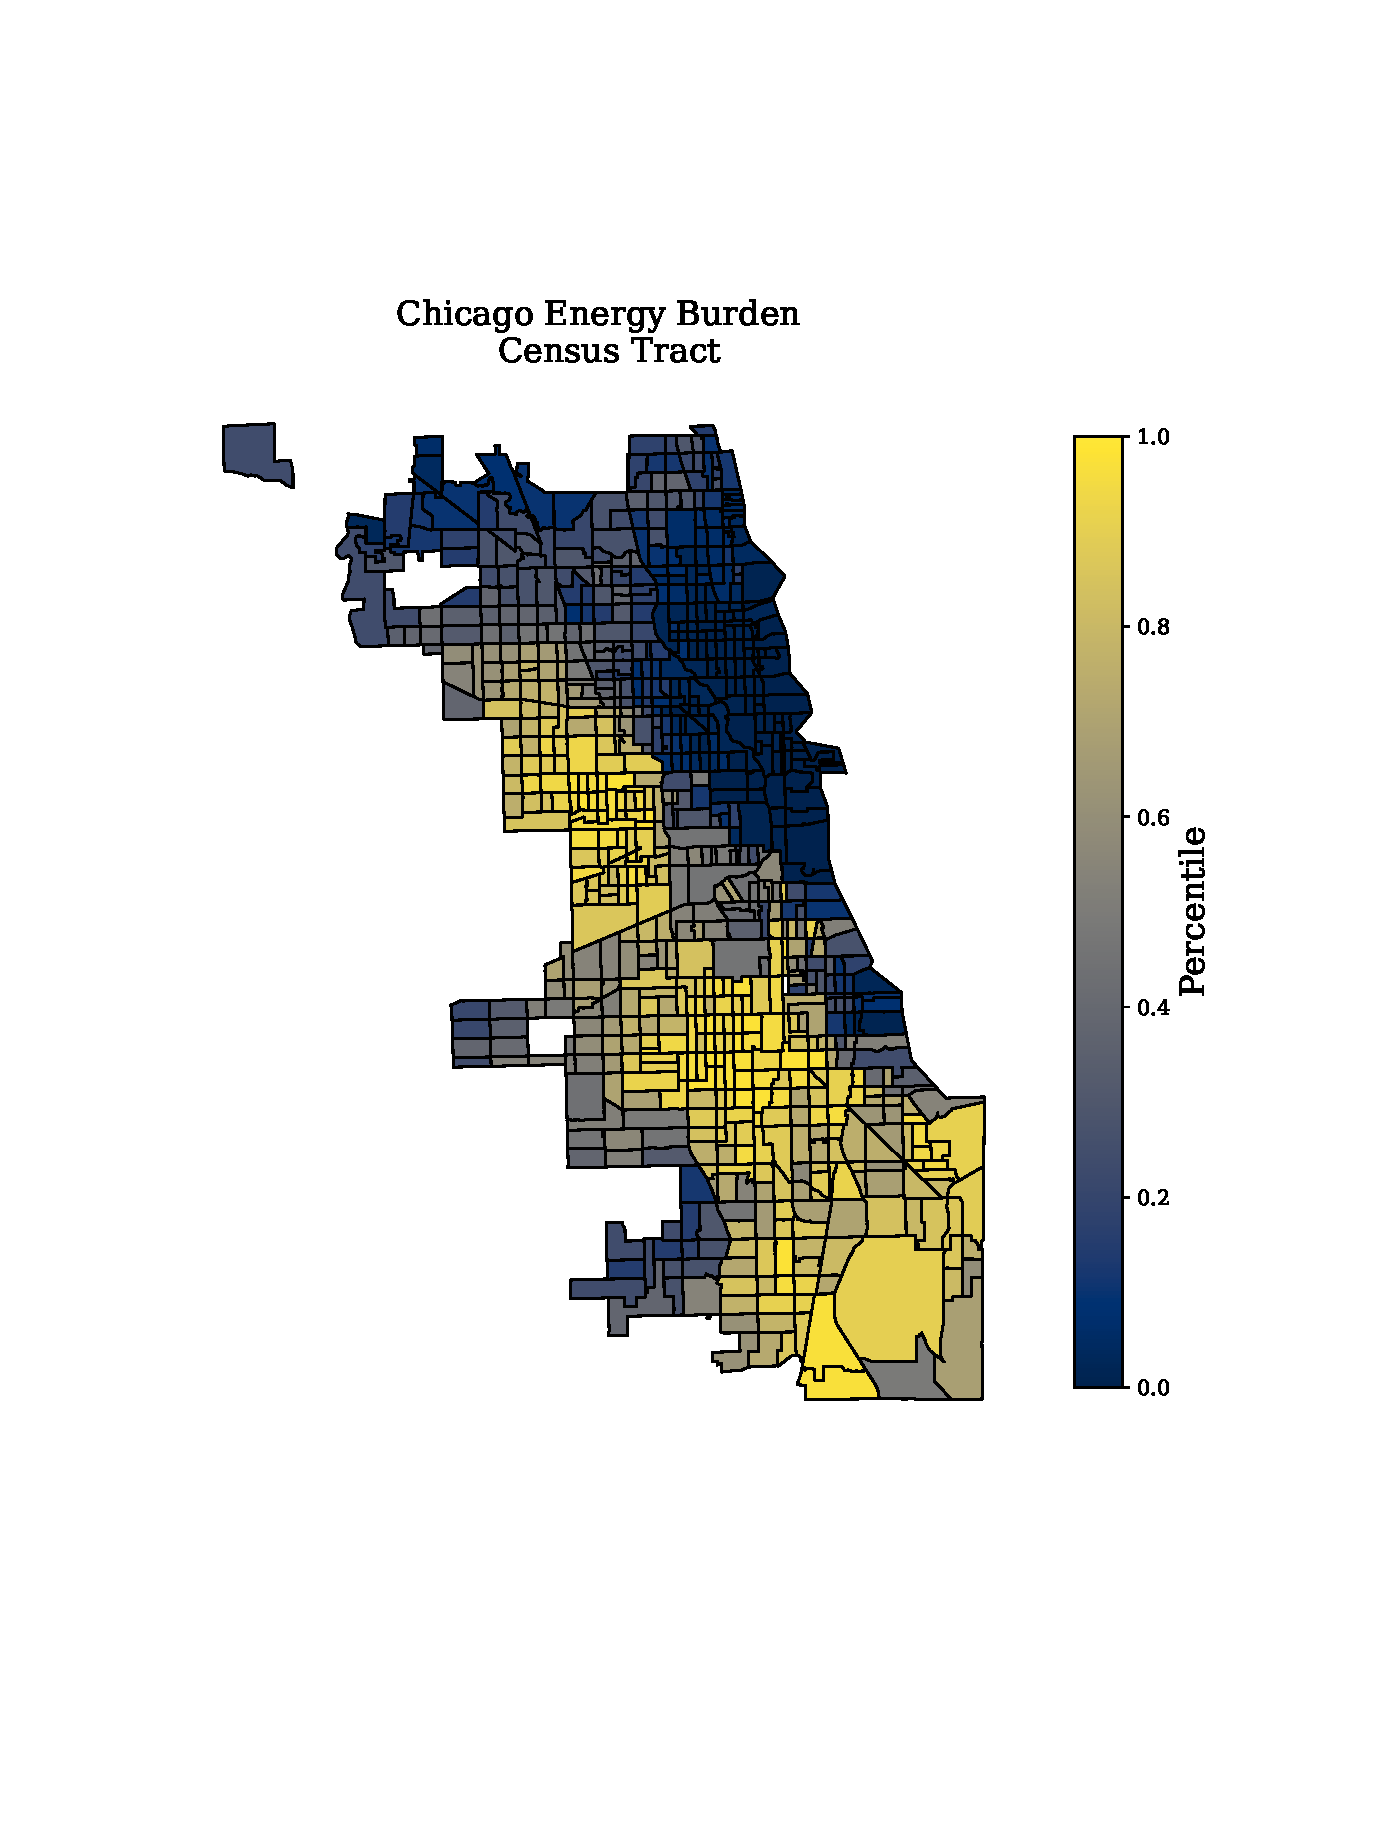
\includegraphics[width=\columnwidth]{energy_burden}
      \vspace*{-2cm}
      \caption{Energy burden throughout Chicago as a percentile. A region in the zeroth
      percentile has the least energy burden and a region in the 100th percentile has
      more energy burden than any other region.}
    \end{center}
\end{figure}

\subsubsection{Tree Canopy}

Urban tree cover effectively mitigate land surface temperatures in cities
\cite{loughner_roles_2012, schwaab_role_2021, mcdonald_tree_2021}. Tree canopy
reduces temperature by preventing ground heat storage through shade and encouraging
evapotranspiration \cite{mcdonald_tree_2021}. Thus, areas with greater tree cover
are less vulnerable heatwaves. Figure \ref{fig:tree_census} shows the distribution
of trees in Chicago from the Morton Arboretum Tree Census \cite{kua_chicago_2020}.

\begin{figure}[H]
  \label{fig:tree_census}
    \begin{center}
      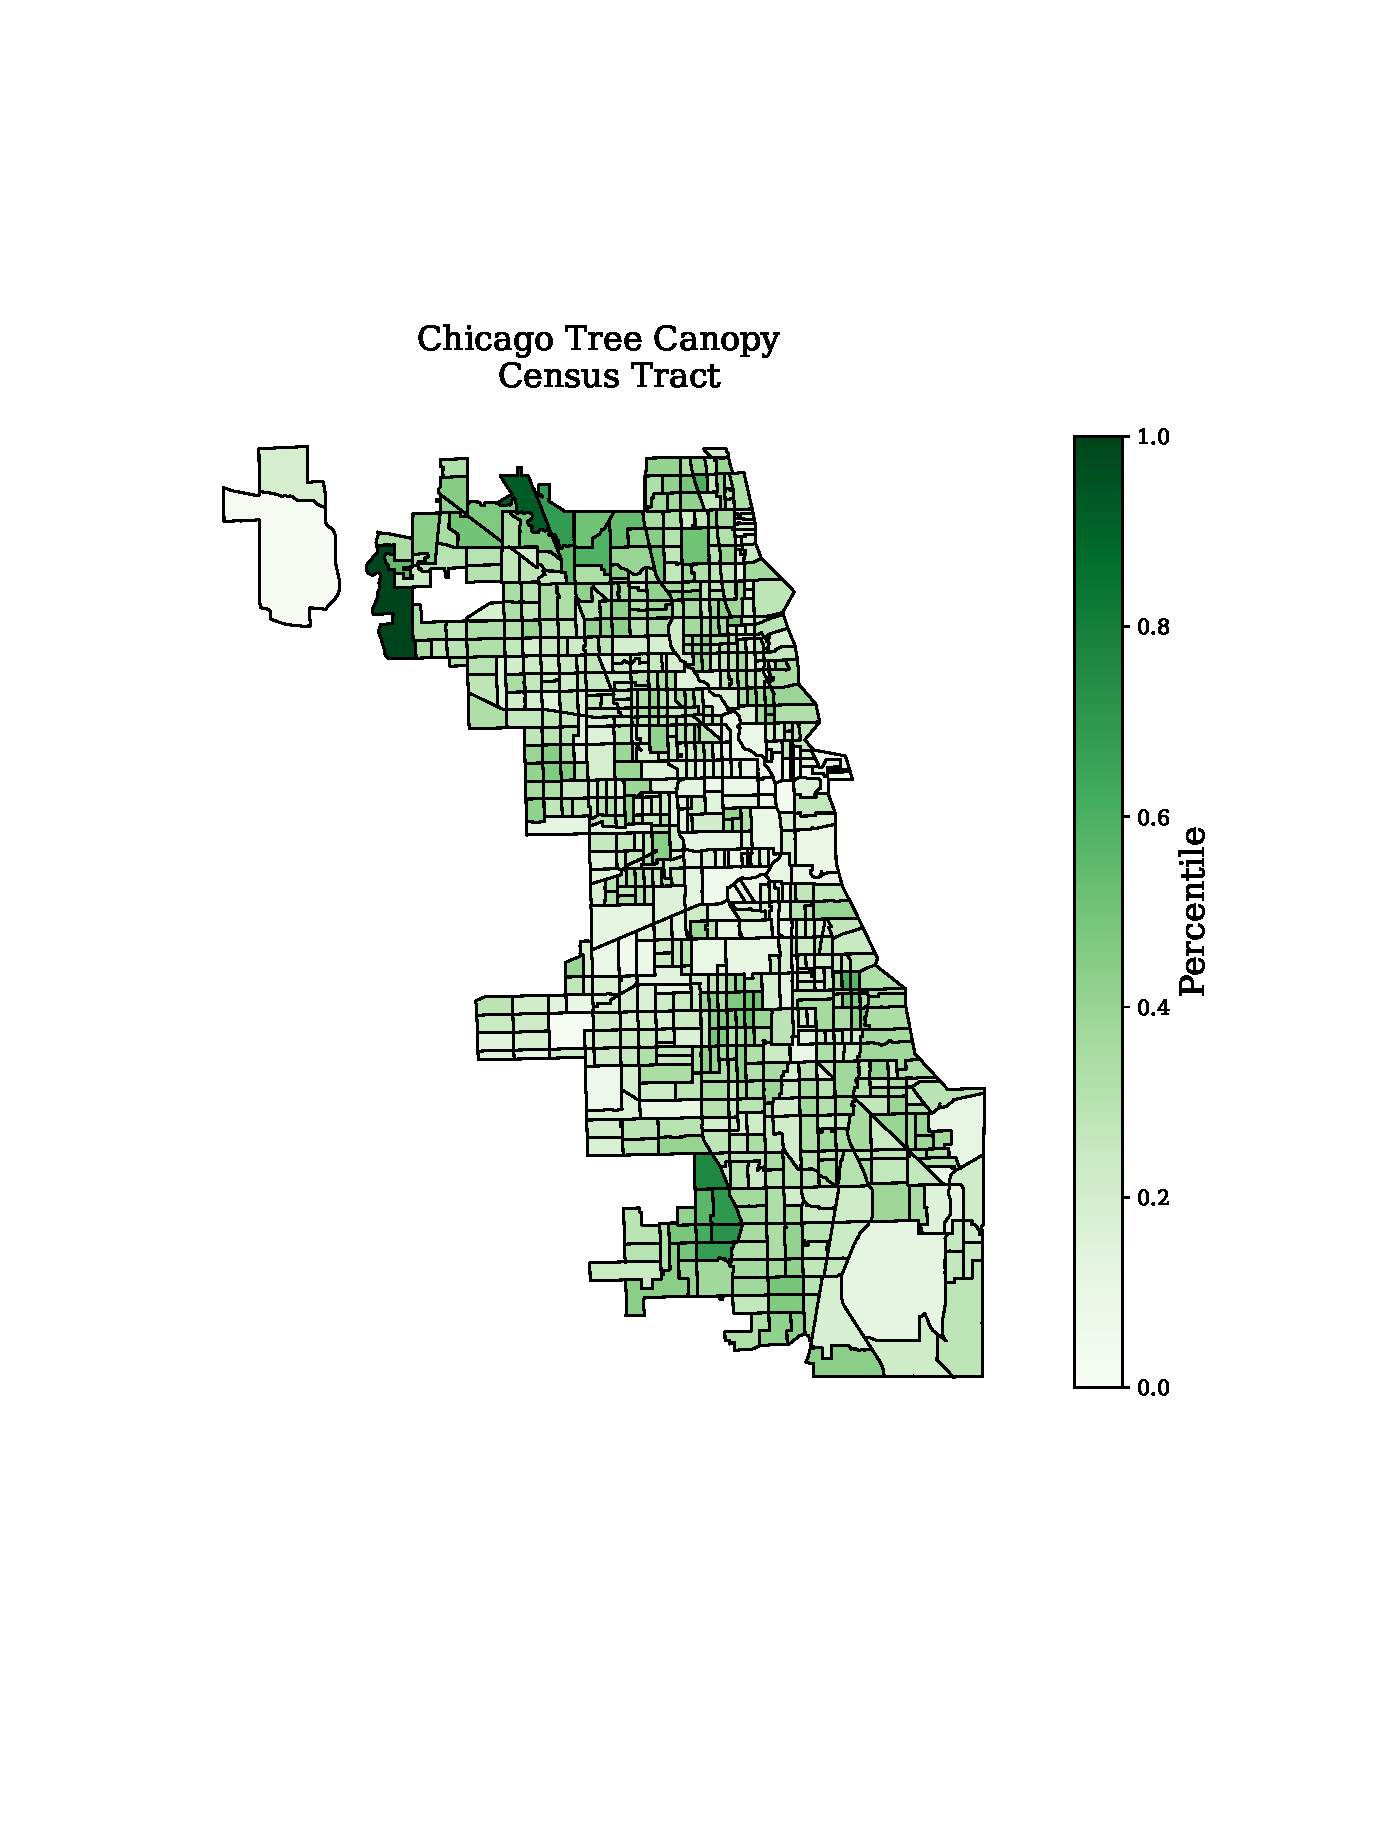
\includegraphics[width=\columnwidth]{tree_canopy}
      \vspace*{-2cm}
      \caption{Distribution of trees in Chicago by percentile. A region in the zeroth
      percentile has the least tree canopy and a region in the 100th percentile has
      more tree cover than any other region.}
    \end{center}
\end{figure}


\section{Results}
\label{section:results}
\begin{figure}[ht]
    \centering
    \label{fig:equity_map}
    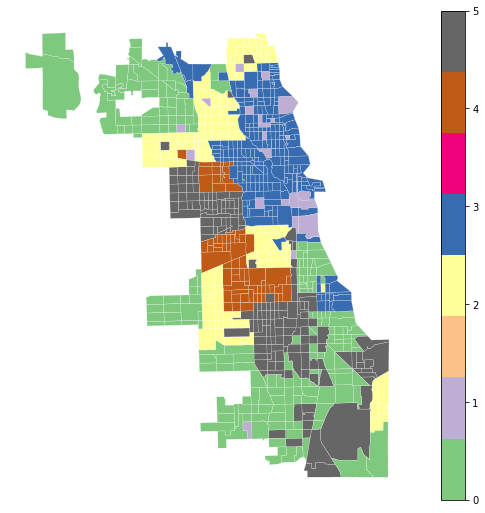
\includegraphics[width=\columnwidth]{cluster_map}
\end{figure}

\section{Discussion}
\label{section:discussion}
\input{discussion}

\section{Conclusion}

% \bibliography
\section*{References}
\bibliographystyle{unsrt}
\bibliography{bibliography}

 \end{document}
